\fancyhead[LO,CE]{Chapter: \thechapter| Analyse et Conception }
 \section*{Introduction}

  
Dans ce chapitre nous aborderons une description générale de notre application, ensuite nous mettons en évidence le côté conceptuel de nos applications qui constitue une étape fondamentale qui précède l’implémentation, cette étape permet de détailler les différents diagrammes et scénarios à implémenter dans la phase suivante. Ceci permettra de mieux comprendre nos applications. Nous avons utilisé une démarche générale basée sur \ac{up} qui utilise  \ac{uml}. 

Dans cette démarche, les diagrammes UML utilisés sont les suivants : Diagramme de cas d’utilisation, le diagramme de classes et le diagramme d'activité sont modélisés à l’aide de l’outil \textit{\textbf{Lucidchart}} .



 \section{Unified Modeling Language (UML):}
 Dans ce qui suit, nous allons donner une brève description d’UML.
 \subsection{ Définition UML }
 L’OMG définit l’UML comme un langage visuel dédié à la spécification, la construction et la documentation des artéfacts d’un système logiciel. Aussi la façon dont tout le monde modélise non seulement la structure de l’application, le comportement et l’architecture, mais aussi des processus d’affaires et la structure des données. Ce langage est conçu pour modéliser divers types de systèmes et de taille quelconque. Il possède une approche entièrement objet couvrant tout le cycle de développement. Le système est décomposé en un ensemble d’objets collaborant \parencite{uml}.
 
 \subsection{Contenu UML}
 
 L’UML comporte 13 diagrammes qui se répartissent en deux catégories \parencite{uml}. Nous ne mentionnons que les diagrammes que nous utilisons, 
 
 \subsubsection{Diagramme structurel : }
 \begin{itemize}
 \item \textbf{Diagramme de classes (Class Diagram) : }ce diagramme décrit la structure statique du système, il définit les classes, leurs attributs et leurs relations. Il est considéré comme le diagramme le plus important.
  \item  \textbf{Diagramme de paquetages (Package Diagram) : }définit les dépendances entres les paquets (groupement d’éléments UML) constituant un modèle. 
 \end{itemize}
 
 
  \subsubsection{Diagramme comportemental  : }
 
  \begin{itemize}
 	\item \textbf{Diagramme de cas d’utilisation (Use Case Diagram) : } pour décrire les besoins des utilisateurs. 
 	\item  \textbf{Diagramme de séquence(Sequence Diagram):}  décrit comment chaque objet interagit avec l’autre et dans quel ordre, sur un axe temporel donné. Ce diagramme sont associés aux diagrammes de cas d’utilisation.
 	. 
 \end{itemize}



\section{Identification des objectifs}
\comment{
Au début du projet, nous nous sommes concentrés sur les besoins qui pourraient normalement être considérés comme un système général et nous avons interrogé les ingénieurs de la société nationaux de retraités    "CNR", qui ont exprimé des besoins importants. 
 
 
 Nos entretiens ont été complétés en suivant les étapes ci-dessous
 
\textbf{ Étape 1:} Choisir les entretiens Afin d'identifier les besoins, nous avons contacté des personnes pouvant fournir des informations utiles et fournir des explications. Les personnes responsables de la production des différentes unités ou entreprises sont les plus appropriées pour répondre à nos questions.
 
\textbf{Étape 2:}
Planification du développement du programme À ce stade de la planification des entretiens, nous avons étudié deux points essentiels:

- Déterminer le contexte général de l'entretien : "CNR",

- Réglage de la date et de l'heure de l'entretien (date). 

\textbf{ Étape 3:} Préparez-vous pour l’entrevue Préparez les questions de développement et les supports pour un processus sans faille (stylos, cartons de réponses, papiers blancs supplémentaires, clé USB).


\textbf{ Étape 4:} Conduisez l’entretien: Commencez le processus d’entretien en vous présentant d’abord, puis en présentant brièvement notre projet, puis en passant l’entretien en interrogeant la personne concernée et en enrichissant sa conversation d’observations et de questions. Intermédiaire.
 
\textbf{ Étape 5:} Après l'entretien Après avoir pris les informations collectées et conclu l'entretien, nous avons décidé de procéder à d'autres entretiens en développant et en nous réunissant à chaque fois.
 
 
 Sur la base de ces entretiens et de l'entretien avec l'enseignant, nous avons pu identifier les spécifications suivantes:
}
 \subsection{Spécifications fonctionnelles }
  Le système doit permettre à l’administrateur  de:
 \begin{enumerate}
\item  	    Générer le modèle. 
\item  	    Gérer Sous-direction. 
\item  	    Gérer les service.
\item  	    Gérer workflow pour les dossier.  
\item  	    Gérer les tâches des service.  
\item  	    Gérer les utilisateur. 
\item  	    Consulte les historique  et la recherche par tâche. 
\item  	    Consulte les historique  et la recherche par dossier et les jours pour chaque tâche. 
\item  	    Consulte bordereau. 
 \end{enumerate}
 Le système doit permettre à l’utilisateur   de :
 \begin{enumerate}
\item  	    Gérer les dossier. 
\item  	    Activé le dossier.    
\item  	    Finir le traitement des dossiers par tâche.    
\item  	    Gérer les  bordereaux.  
\item  	    Accepte le  bordereau.  
\item  	    Refuse  le  bordereau.  
\item  	    Imprimer le  bordereau.  

 \end{enumerate}
 
 
 
 
  \subsection{Spécifications techniques }
 
 
 
  \begin{enumerate}
 	\item  	   Le système doit être déployé sur le cloud.  
 	\item  	   La configuration et la génération  de code dynamique.  
 	\item  	  Modélisation d'un workflow Administratif via une interface graphique simple et utile. 
 
 	
 \end{enumerate}
 
 
 
 
 
 
 
 
 
 
 
\subsection{ Diagramme de cas d’utilisation }
 
  \subsubsection{ les acteurs de système  }
 
Un acteur représente l'abstraction d'un rôle joué par des entités externes (utilisateur, dispositifs matériels ou autres système) qui interagit directement avec le système (réception d’informations, etc.). Pour notre application, on a trois acteurs : le premier acteur c'est l'administrateur et le deuxième c'est utilisateur de la réception et le troisième c'est l'utilisateur simple.
\begin{table}[H]

	   
	\begin{tabular}{|l|l|l|}
		\hline
		\multicolumn{1}{|l|}{Acteur} & Type Acteur & Descriptions \\ \hline
	Administrateur	 &  & S’authentifier \\ \cline{3-3} 
		&  &Généré le modèle\\ \cline{3-3} 
		&  & Gérer Sous-direction \\ \cline{3-3} 
	 	&  & Gérer les Services \\ \cline{3-3} 	
	 	&  & Gérer les Tâches \\ \cline{3-3} 
 
		& Acteur Principale & Gérer   le Workflow   \\ \cline{3-3} 
				&  &Consulter les bordereaux   \\ \cline{3-3} 
						&  &Consulter les historiques des dossiers\\ \cline{3-3} 
								&  & Gérer les Utilisateurs \\ \hline 
		
  
			Utilisateur réception	 	&Acteur Principal & Créer et Gérer les dossiers  \\ \cline{3-3}  
		&  & Activé les dossiers et ajoute sur wf \\ \hline
 
		Utilisateur Simple	&  & finir le traitement de dossier  \\ \cline{3-3} 
		&  Acteur Principal& Gérer les bordereaux  \\ \cline{3-3} 
		&  &Gérer les historiques des dossiers\\ \hline 
	\end{tabular}
	   	\label{fig:as}
        \caption{Les acteurs de système}
\end{table}
 
 \subsubsection{ Cas d’utilisation }

Le diagramme des cas d’utilisation suivante illustre les fonctionnalités qu’un simple utilisateur du système, également l’administrateur, peut faire. Ce diagramme a été inspiré des spécifications citées ci-dessus :
 
 \begin{figure}[H]
 	\centering
 	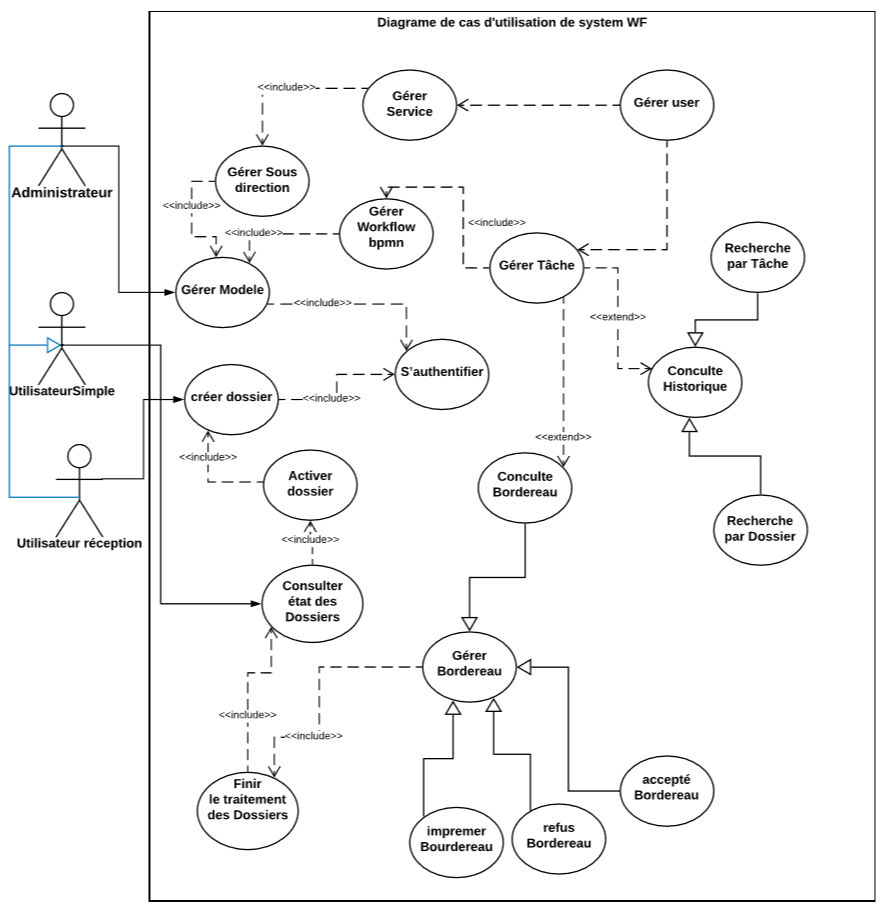
\includegraphics[width=1\linewidth,height=0.8\paperheight]{usercase2}
 	\caption{Diagramme de Cas d’utilisation}
 	\label{fig:usercase2}
 \end{figure}
 
 \subsection{ Documentation des cas d’utilisation fonctionnels }
Nous détaillerons chaque cas d'utilisation avec une description brève et spécifions les acteurs principaux et les acteurs secondaires, ainsi que les postconditions et les préconditions pour le faire sont la séquence principale et la séquence alternative.

 \subsubsection{ S’authentifier }
 \begin{table}[H]
 	\centering
 	\begin{tabular}{|l|} 
 		\hline
 	\textbf{	CU :} S’authentifier     \\  	\hline
 		\textbf{ID:}1         \\  		\hline
 		\begin{tabular}[c]{@{}l@{}}\textbf{Description brève :} chaque utilisateur doit s’authentifier\\ auprès de l’application afin de pouvoir  utiliser les fonctionnalités\\ du système. \end{tabular}          \\ 
 		\hline
 		\textbf{Acteurs primaires : }utilisateur, administrateur   \\ 
 		\hline
 		Acteurs secondaires :                                                                                                                                                                                                                                                                                                                                                                                                                                                                                                                                                                                                                                                                                                                                                                             \\ 
 		\hline
 		\begin{tabular}[c]{@{}l@{}}\textbf{Pré-conditions :}\\ – La connexion auprès du serveur d’applications doit être réussite.
 			\\ – L’utilisateur  doit être enregistré dans le système. \end{tabular}                                                                                                                                                                                                                                                                                                                                                                                                                                                                                                                                                                                                           \\ 
 		\hline
 		\begin{tabular}[c]{@{}l@{}}\textbf{Enchainement principal : }Ce cas d’utilisation commence lorsqu’un\\ utilisateur souhaite accéder à   l’application. 
 			\\ 1. L’utilisateur saisit le lien de l’application dans barre d’adresse du navigateur. 
 			\\ 2. Le serveur répond à l’utilisateur en renvoyant une page  d’authentification.
 			\\ 3. L’utilisateur saisit son nom et son mot de passe et en appuyant \\ sur  “S'identifier” (Figure\ref{fig:login}).
 			\\ 4. Le serveur vérifie la validité du nom d’utilisateur et du mot de passe. 
 			\\ 5. Le serveur envoie une page d’accueil de l’application à l’utilisateur concerné. \end{tabular}     \\ 
 		\hline
 		Post-conditions : L’utilisateur est connecté.                                                                                     \\ 
 		\hline
 		\begin{tabular}[c]{@{}l@{}}Enchainement alternatif :  \\\begin{tabular}{@{\labelitemi\hspace{\dimexpr\labelsep+0.5\tabcolsep}}l} E1 : La page d’authentification n’apparaît pas à l’utilisateur.\end{tabular}\\ * L’enchainement démarre   après le premier point de l’enchainement principal. \\ * Le serveur envoie un message d’erreur à  l’utilisateur. \\\begin{tabular}{@{\labelitemi\hspace{\dimexpr\labelsep+0.5\tabcolsep}}l} E2 : Le nom d’utilisateur ou/et le mot de passe ne sont pas validés.\end{tabular}  
 			\\
 			* Le serveur envoie un message d’erreur à l’utilisateur.
 			
 			\\ * Le serveur demande à l’utilisateur se ressaisit le nom d’utilisateur et le mot de passe. \end{tabular}  \\
 		\hline
 	\end{tabular}
 
 
 \end{table}







\subsubsection{Créer circuit Workflow}
\begin{table}[H]
	\begin{tabular}{|l|}
		\hline
		\textbf{CU : }Créer circuit Workflow\\ \hline
		\textbf{ID }: 12 \\ \hline
		\textbf{Description brève :}L'administrateur Crée un circuit de Workflow pour \\l'enchainement des dossiers \\ \hline
		\textbf{Acteurs primaires :} L'administrateur  \\ \hline
		\textbf{Acteurs secondaires :}\\ \hline
		\textbf{Pré-conditions :}  L'administrateur doit être connecté \\ \hline
		\begin{tabular}[c]{@{}l@{}}\textbf{Enchainement principal :} Un circuit Workflow est créé pour les dossiers  et \\la création des tâches sur la base de donnée normale. \end{tabular} \\ \hline
		\textbf{Post-conditions : }Workflow est défié et les tâches à remplir      \\ \hline
		\begin{tabular}[c]{@{}l@{}}\textbf{Enchainement alternatif : }   \\ \end{tabular} \\ \hline
	\end{tabular}
\end{table}







\subsubsection{Gérer les Services}
\begin{table}[H]
	\begin{tabular}{|l|}
		\hline
		\textbf{CU : }Gérer les Services \\ \hline
		\textbf{ID }: 22 \\ \hline
		\textbf{Description brève :}L'administrateur peut gérer les services à travers la création, \\ la modification et la suppression d'un ou plusieurs services. \\ \hline
		\textbf{Acteurs primaires :} L'administrateur  \\ \hline
		\textbf{Acteurs secondaires :}  \\ \hline
		\textbf{Pré-conditions :} L'administrateur doit être connecté  \\ \hline
		\begin{tabular}[c]{@{}l@{}}\textbf{Enchainement principal :}L'administrateur crée un nouveau service au\\ système et peut le modifier.  \end{tabular} \\ \hline
		\textbf{Post-conditions : } le service ajouté sur  la base de donnée (BDD) \\ \hline
		\begin{tabular}[c]{@{}l@{}}\textbf{Enchainement alternatif : }    \\\end{tabular} \\ \hline
	\end{tabular}
\end{table}

\subsubsection{Gérer utilisateur  }
\begin{table}[H]
	\begin{tabular}{|l|}
		\hline
		\textbf{CU : }Gérer utilisateur \\ \hline
		\textbf{ID }: 12 \\ \hline
		\textbf{Description brève :}Un administrateur peut gérer des utilisateurs en créant des \\ comptes  en spécifiant une tâche pour chacun d'eux.  \\ \hline
		\textbf{Acteurs primaires :} L'administrateur  \\ \hline
		\textbf{Acteurs secondaires :}   \\ \hline
		\textbf{Pré-conditions :} L'administrateur doit être connecté   \\ \hline
		\begin{tabular}[c]{@{}l@{}}\textbf{Enchainement principal :} L'administrateur a créé des comptes \\d'utilisateurs. \end{tabular} \\ \hline
		\textbf{Post-conditions : }Comptes d'utilisateurs créés\\ \hline
		\begin{tabular}[c]{@{}l@{}}\textbf{Enchainement alternatif : } \\ \end{tabular} \\ \hline
	\end{tabular}
\end{table}




\subsubsection{Consulter  Historique   }
\begin{table}[H]
	\begin{tabular}{|l|}
		\hline
		\textbf{CU : }Consulter  Historique \\ \hline
		\textbf{ID }: 32 \\ \hline
		\textbf{Description brève :}L'administrateur peut consulter l'historique des dossiers\\ et leur état, ainsi la recherche par dossier ou la recherche par tâche.   \\ \hline
		\textbf{Acteurs primaires :} L'administrateur  \\ \hline
		\textbf{Acteurs secondaires :}   \\ \hline
		\textbf{Pré-conditions :} L'administrateur doit être connecté   \\ \hline
		\begin{tabular}[c]{@{}l@{}}\textbf{Enchainement principal :}
			\\ -L'administrateur sélectionne le dossier ou la  tâche et en appuyant\\ sur rechercher .  
			\\ -Le système  affiche l'état des dossiers.   \end{tabular} \\ \hline
		\textbf{Post-conditions : }Afficher le résultat de la recherche \\ \hline
		\begin{tabular}[c]{@{}l@{}}\textbf{Enchainement alternatif : } \\ \end{tabular} \\ \hline
	\end{tabular}
\end{table}











 \subsubsection{Cas d'utilisation par l'utilisateur réception   }
L'utilisateur de réception fait deux rôles principal : la création et l'activation des dossiers.
  \subsubsection{Créer Dossiers}
 \begin{table}[H]
 	\begin{tabular}{|l|}
 		\hline
 	\textbf{CU : }Créer   Dossiers \\ \hline
 	\textbf{ID }: 2 \\ \hline
 	\textbf{Description brève :} chaque utilisateur peut créer  et enregistrer\\des nouveaux dossiers.\\ \hline
 	\textbf{Acteurs primaires :} utilisateur de réception , \\ \hline
 		\textbf{Acteurs secondaires :} simple utilisateur \\ \hline
 	\textbf{Pré-conditions :} L’utilisateur doit être  connecté au  système. \\ \hline
 		\begin{tabular}[c]{@{}l@{}}\textbf{Enchainement principal :} Ce cas d’utilisation commence lorsqu’un utilisateur\\ souhaite accéder à l’application.
 			\\ 1. L’utilisateur sélectionne d'ajouter nouveau dossier. 
 			\\ 2. système répond à l’utilisateur en affichant un formulaire d'enregistrement.
 			\\ 3. L’utilisateur saisit le code et le nom, le prénom et le numéro de téléphone de \\ propriétaire de dossier.
 			\\ 4. L'utilisateur vérifie le dossier et sélectionne les champs actuels \\en appuyant sur  « Enregistrer ». 
 			\\ 5. Le système envoie une page des dossiers.\end{tabular} \\ \hline
 		\textbf{Post-conditions : }le dossier est enregistré et ajouté dans le système. \\ \hline
 		\begin{tabular}[c]{@{}l@{}}\textbf{Enchainement alternatif : }    \\  \textbf{ E1:} Le code de dossier n'est pas validé ou/et déjà existé.\\   o     Le serveur envoie un message d’erreur à  l’utilisateur. \\   o   Le serveur demande à l’utilisateur se ressaisit le code de dossier.\end{tabular} \\ \hline
 	\end{tabular}
 \end{table}
 
 




\subsubsection{Activer Dossiers}
\begin{table}[H]
	\begin{tabular}{|l|}
		\hline
		\textbf{CU : }Activer Dossiers \\ \hline
		\textbf{ID }: 3 \\ \hline
		\textbf{Description brève :}\\L'utilisateur peut activer le statut du dossier et commencer au  début de \\la tâche "Ajouter au flux de travail", après avoir compléter tous \\les documents de dossier.    \\ \hline
		\textbf{Acteurs primaires :} utilisateur réception , \\ \hline
		\textbf{Acteurs secondaires :} simple utilisateur \\ \hline
		\textbf{Pré-conditions :} Le dossier  doit être enregistré dans le système.\\ \hline
		\begin{tabular}[c]{@{}l@{}}\textbf{Enchainement principal :} \\ 1.   L’utilisateur sélectionne   la liste des dossiers. \\2.      système répond à l’utilisateur en affichant les listes des dossiers \\ \{"toute la liste","liste activée ","liste non activée"\}. \\3.       L’utilisateur sélectionne le dossier \\ 4. le système  répond à l’utilisateur en affichant le détail, et après\\  en appuyant sur "Activer".\\5. le système vérifie ID "code" de dossier et active leur état \end{tabular} \\ \hline
		\textbf{Post-conditions : }le dossier  est activé dans la premier tâche.  \\ \hline
		\begin{tabular}[c]{@{}l@{}}\textbf{Enchainement alternatif : } \end{tabular} \\ \hline
	\end{tabular}
\end{table}



\subsubsection{Cas d'utilisation par l'utilisateur simple  }
l'utilisateur fait un rôle principal : consulter l'état du dossier pour finir le traitement créer des bordereaux pour transférer les dossiers (imprimer et refuser ou accepter les bordereaux).
 
 
\subsubsection{Consulter l'état des Dossiers}
\begin{table}[H]
	\begin{tabular}{|l|}
		\hline
		\textbf{CU : }Consulter l'état  des dossiers \\ \hline
		\textbf{ID }: 4 \\ \hline
		\textbf{Description brève :}L'utilisateur peut visualiser le statut des dossiers en cours \\ de traitement  en fonction de sa tâche et voir tous les dossiers envoyés par une \\autre tâche.     \\ \hline
		\textbf{Acteurs primaires :} utilisateur  \\ \hline
		\textbf{Acteurs secondaires :}  \\ \hline
		\textbf{	Pré-conditions :} 
\\ - Le dossier doit être Activé dans le système.
\\ - L’utilisateur doit être connecté au système.
		\\ \hline
		\begin{tabular}[c]{@{}l@{}}\textbf{Enchainement principal :} \\ 1. L’utilisateur sélectionne le statut des dossiers.
			\\ 2.Le système répond à l’utilisateur en affichant les listes des dossiers au cours de traitement\\ ou les nouveaux dossiers envoyés \end{tabular} \\ \hline
		\textbf{Post-conditions : }L'utilisateur visualise le statut des dossiers en fonction de sa tâche.\\ \hline
		\begin{tabular}[c]{@{}l@{}}\textbf{Enchainement alternatif : } \end{tabular} \\ \hline
	\end{tabular}
\end{table}


\comment{
\subsubsection{Finir le traitement  des Dossiers}
\begin{table}[H]
	\begin{tabular}{|l|}
		\hline
		\textbf{	CU : }Finir le traitement  des Dossier \\ \hline
		\textbf{	ID }: 5 \\ \hline
		\textbf{	Description brève :}L'utilisateur peut sélectionner une liste des dossiers et finir\\ leur traitement \\ \hline
		\textbf{Acteurs primaires :} utilisateur  \\ \hline
		\textbf{Acteurs secondaires :}  \\ \hline
		\textbf{Pré-conditions :} 
		\\ - Le dossier doit être Activé dans la tâche de l'utilisateur. 
		\\ - L’utilisateur doit être connecté au système. 
		\\ \hline
		\begin{tabular}[c]{@{}l@{}}\textbf{Enchainement principal :} 
			\\ 1. L’utilisateur sélectionné la liste des dossiers pour finir le traitement en payent \\sur "terminer", \\ 2. système répond à l’utilisateur et terminer le traitement des dossiers par \\ changer état et la date fin de traitement. \end{tabular} \\ \hline
		\textbf{Post-conditions : }L'utilisateur   finissait le traitement   des dossiers par sa tâche. \\ \hline
		\begin{tabular}[c]{@{}l@{}}\textbf{Enchainement alternatif : } \end{tabular} \\ \hline
	\end{tabular}
\end{table}


}



\subsubsection{Gérer Bordereau}
\begin{table}[H]
	\begin{tabular}{|l|}
		\hline
		\textbf{	CU : }Gérer Bordereau   \\ \hline
		\textbf{	ID }: 6 \\ \hline
		\textbf{	Description brève :}L'utilisateur peut sélectionner une liste des dossiers et \\gère un bordereau. \\   \hline
		\textbf{ Acteurs primaires :} utilisateur  \\ \hline
		\textbf{Acteurs secondaires :}  \\ \hline
		\textbf{	Pré-conditions :} 
		\\ - Le dossier doit être traité dans la tâche de l'utilisateur.
		\\ - L’utilisateur doit être connecté au système. 
		\\ \hline
		\begin{tabular}[c]{@{}l@{}}\textbf{Enchainement principal :} \\ 1. L’utilisateur sélectionne la liste des dossiers pour la transférer à \\la tâche  suivante.\\ 2.Le système répond à l’utilisateur et crée un nouveau bordereau et affiche la liste\\ de bordereau correspondant à leur tâche. 
			\\ 3. L’utilisateur peut imprimer et accepter ou refuser le bordereau.   \end{tabular} \\ \hline
		\textbf{Post-conditions : } L'utilisateur crée un bordereau et transfert les dossiers, \\si le bordereau est accepté par la validation d'un utilisateur de la tâche reçu.  \\ \hline
		\begin{tabular}[c]{@{}l@{}}\textbf{Enchainement alternatif : }  \\
	\textbf{E1: }bordereau refusé:
\\ * renvoyer à la tâche précédent tous les dossiers.   
	
 \end{tabular} \\ \hline
	\end{tabular}
\end{table}
 
 \section{ Représentation des informations }
 \subsection{Diagramme de Classe}
\begin{figure}[H]
	\centering
	\includegraphics[width=1\linewidth,height=0.7\paperheight]{images/class01}
	\caption{Diagramme de Classe}
	\label{fig:class01}
\end{figure}

 % \subsubsection{Conception détaillée} 
Nous allons définir pour chaque classe ses attributs et leurs types, ainsi que les méthodes qu’elle offre. Dans le but d’alléger le rapport, nous allons cité que les classes essentiels que nous avons conçues.
 
 
 \subsubsection{La classe Dossier}
 \begin{table}[H]
 	\centering\setlength\tabcolsep{1cm}
 	
 	\begin{tabular}{|l|l|l|}
 		\hline
 		\textbf{Attribut}  & \textbf{Type} & \multicolumn{1}{l|}{\textbf{Méthodes}} \\ \hline
 		
 		id & long & getId() et setId()\\ \cline{1-2}
 		nom & String & getNom() et setNom()\\ \cline{1-2}
 		prenom & String & getPrenom() et setPrenom()\\ \cline{1-2}
 		tlphon & String & getTlphon() et setTlphon()\\ \cline{1-2}
 		ch1 & boolean  & getCh1() et setCh1()\\ \cline{1-2}   
 		ch2 & boolean  & getCh2() et setCh2() \\ \cline{1-2}
 		ch3 & boolean  & getCh3() et setCh3() 
 		\\ \hline
 	\end{tabular}
 	\caption{La classe Bordereau}
 	\label{fig:class8}
 \end{table}
 
 

\subsubsection{La classe Service}
\begin{table}[H]
	\centering
	\begin{tabular}{|l|l|l|}
		\hline
		\textbf{Attribut}  & \textbf{Type} & \multicolumn{1}{l|}{\textbf{Méthodes}} \\ \hline
		
		id & long & getId() et setId()\\ \cline{1-2}
		nom & String  & getNom() et setNom() \\ \cline{1-2}
				sous-Direction & Sous-Direction  & getSous-Direction() et setSous-Direction() \\ \cline{1-2}
		myTasks	& $ List<MyTask> $ & getMyTasks() et setMyTasks()   \\ \hline
	\end{tabular}
	\caption{La classe Service}
\label{fig:class2}
\end{table}


\subsubsection{La classe MyTask}
\begin{table}[H]
	\centering
	\begin{tabular}{|l|l|l|}
		\hline
		\textbf{Attribut}  & \textbf{Type} & \multicolumn{1}{l|}{\textbf{Méthodes}} \\ \hline
		
		id & long & getId() et setId()\\ \cline{1-2}
		nom & String  & getNom() et setNom() \\ \cline{1-2}
			idTask & String & getIdTask() et setIdTask()\\ \cline{1-2}
		services & Service  & getService() et setService() \\ \cline{1-2}
				users	& $ List<User> $ & getUsers() et setUsers()   \\ \cline{1-2}	
				
		nextMyTasks	& $ List<NextMyTask> $ & getNextMyTasks() et setNextMyTasks()   \\ \hline
	\end{tabular}
	\caption{La classe MyTask}
\label{fig:class3}
\end{table}




\subsubsection{La classe Utilisateur "User"}
\begin{table}[H]
	\centering\setlength\tabcolsep{1cm}
	
	\begin{tabular}{|l|l|l|}
		\hline
		\textbf{Attribut}  & \textbf{Type} & \multicolumn{1}{l|}{\textbf{Méthodes}} \\ \hline
		
		id & long & getId() et setId()\\ \cline{1-2}
		nom & String & getNom() et setNom()\\ \cline{1-2}
			prenom & String & getPrenom() et setPrenom()\\ \cline{1-2}
						tlphon & String & getTlphon() et setTlphon()\\ \cline{1-2}
		myTask & MyTask  & getMyTask() et setMyTask()   \\ \hline
	\end{tabular}	\caption{La classe Bordereau}
\label{fig:class6}
\end{table}


\subsubsection{La classe NextTask}
\begin{table}[H]
	\centering\setlength\tabcolsep{1cm}
	
	\begin{tabular}{|l|l|l|}
		\hline
		\textbf{Attribut}  & \textbf{Type} & \multicolumn{1}{l|}{\textbf{Méthodes}} \\ \hline
		
		id & long & getId() et setId()\\ \cline{1-2}
		idTask & String & getIdTask() et setIdTask()\\ \cline{1-2}
		myTask & MyTask  & getMyTask() et setMyTask()   \\ \hline
	\end{tabular}
	\caption{La classe Bordereau}
	\label{fig:class5}
\end{table}






\subsubsection{La classe  Sous-Direction}
\begin{table}[H]
	\centering\setlength\tabcolsep{0.8cm}
	\begin{tabular}{|l|l|l|}
		\hline
		\textbf{Attribut}  & \textbf{Type} & \multicolumn{1}{l|}{\textbf{Méthodes}} \\ \hline
		
		id & long & getId() et setId()\\ \cline{1-2}
		nom & String  & getNom() et setNom() \\ \cline{1-2}
		services	& $ List<Service> $ & getServices() et setServices()   \\ \hline
	\end{tabular}	\caption{La classe Sous-Direction}
	\label{fig:class1}
\end{table}


\subsubsection{La classe Historique}
\begin{table}[H]
	\centering\setlength\tabcolsep{1cm}
	
	\begin{tabular}{|l|l|l|}
		\hline
		\textbf{Attribut}  & \textbf{Type} & \multicolumn{1}{l|}{\textbf{Méthodes}} \\ \hline
		
		id & long & getId() et setId()\\ \cline{1-2}
		dateD & Date() & getDateD() et setDateD()\\ \cline{1-2}
		
				dateF & Date() & getDateF() et setDateF()\\ \cline{1-2}
				
				dossier & Dossier & getDossier() et setDossier()\\ \cline{1-2}
				
					user & User & getUser() et setUser()\\ \cline{1-2}
					
					etat & boolean & isEtat() et setEtat()\\ \cline{1-2}
				transfert & boolean & isTransfert() et setTransfert()\\ \hline
	\end{tabular}
	\caption{La classe Bordereau}
\label{fig:class10}
\end{table}
 
   
   


\subsubsection{La classe Role}
\begin{table}[H]
	\centering\setlength\tabcolsep{1.2cm}
	
	\begin{tabular}{|l|l|l|}
		\hline
		\textbf{Attribut}  & \textbf{Type} & \multicolumn{1}{l|}{\textbf{Méthodes}} \\ \hline
		
		id & long & getId() et setId()\\ \cline{1-2}
		nom & Date() & getNom() et setNom()\\ \hline
	\end{tabular}	\caption{La classe Bordereau}
	\label{fig:class7}
\end{table}

\subsubsection{La classe ListDossier}
\begin{table}[H]
	\centering\setlength\tabcolsep{0.8cm}
	
	\begin{tabular}{|l|l|l|}
		\hline
		\textbf{Attribut}  & \textbf{Type} & \multicolumn{1}{l|}{\textbf{Méthodes}} \\ \hline
		
		id & long & getId() et setId()\\ \cline{1-2}
		bordereau & Bordereau & getBordereau() et setBordereau()\\ \cline{1-2}
		historique & Historique & getHistorique() et setHistorique()\\   \hline
	\end{tabular}
	\caption{La classe Bordereau}
	\label{fig:class9}
\end{table}

\subsubsection{La classe Bordereau}
\begin{table}[H]
	\centering\setlength\tabcolsep{1cm}
	
	\begin{tabular}{|l|l|l|}
		\hline
		\textbf{Attribut}  & \textbf{Type} & \multicolumn{1}{l|}{\textbf{Méthodes}} \\ \hline
		
		id & long & getId() et setId()\\ \cline{1-2}
		dateD & Date() & getDateD() et setDateD()\\ \cline{1-2}
		
		user & User & getUser() et setUser()\\ \cline{1-2}
		myTask1 & MyTask  & getMyTask1() et setMyTask1()   \\ \cline{1-2}
		myTask2 & MyTask  & getMyTask2() et setMyTask2() \\ \cline{1-2}  
		etat & String[] & getEtat() et setEtat()\\ \cline{1-2}
		historique & Historique & getHistorique() et setHistorique()\\ \hline
	\end{tabular}
	\caption{La classe Bordereau}
	\label{fig:Bordereau}
\end{table}

\subsection{Diagramme d' activité  }

À partir de deux diagrammes, cas d'utilisation et de classes,  on va exprimer  le diagramme d'activité qui  montre l'interaction des  utilisateurs   en fonction de leurs rôles dans le système en général.(figure \ref{fig:dactiviti})

\subsubsection{Rôles de l'acteur administrateur: }
l'interaction de l'acteur administrateur avec le système, il faut d'abord de connecter au système, puis créer et définir le modèle par la spécification de nom et les champs de dossier pour la génération de codes et lancer un nouveau micro-service et le déployer sur le Cloud par leur nom de service spécifié, ensuite il peut gérer les sous-directions et les services, le modèle de workflow par "BPMN" pour gérer les tâches, gérer les comptes d'utilisateurs, et enfin il  consulte les bordereaux qui sont géré par les utilisateurs et de même consulter l'historiques.
\subsubsection{Rôles de l'acteur utilisateur réception : }
L'interaction de l'utilisateur réception, il faut déjà créer ses comptes par l'administrateur pour connecter au système.  L'utilisateur peut gérer les dossiers par la création des nouveaux dossiers sur la réception et vérifier les champs de chaque dossier, ensuite il peut activer les dossiers c-à-d lancer le  traitement de dossier.

\subsubsection{Rôles de l'acteur utilisateur simple : } 
Après l'authentification au système,  l'utilisateur se connecter sur leur tâche et il peut voir tous les dossiers en attente qui sont en cours de traitement et consulter les bordereaux qui déjà reçu par une autre tâche, l'utilisateur peuvent finir le traitement de dossier par leur tâche, il peut aussi gérer un nouveau bordereau pour transférer une liste des dossiers vers d'autres tâches et de gérer l'historique des dossiers.
   
   \begin{figure}[H]
   	\centering
   	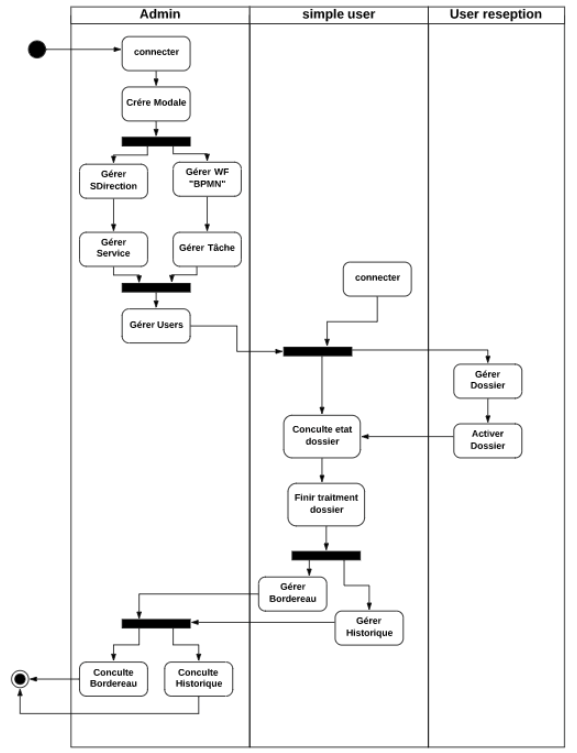
\includegraphics[width=1\linewidth,height=0.6\paperheight]{Dactiviti}
   	\caption{Diagramme d'activité qui  montre interaction des  utilisateurs   en fonction de leurs rôles dans le système en général.}
   	\label{fig:dactiviti}
   \end{figure}
     
   \section{Conclusion}
   
   Dans ce chapitre nous avons fait une étude de notre système logiciel en utilisant la modélisation UML après la spécification des besoins. 
     
        Dans le chapitre suivant nous allons expliqué la phase de réalisation du système, son intégration et son déploiement sur le  cloud par les micro-services, tout en respectant les directives de la conception.
    
    